\chapter{Electromagnetism}

\section{Electrostatics}

\begin{definition}[Electric charge] A scalar quantity that can describe an object. It can be positive or negative
\end{definition}

\begin{definition}[Elementary charge ($e$)] The smallest possible charge $e \approx 1.6 * 10^{-19} \, \Coulomb$.
\end{definition}

\subsection{Charging}

\begin{procedure}[Charging by friction] Rub two nonconductive objects together. The one with the greater electron affinity (electronegativity) becomes negatively charged.
\end{procedure}

\begin{procedure}[Polarization] When two objects near each other, their charge distributions will change in order to ensure that similar charges in the different objects don't get too near each other.
\end{procedure}

% TODO: Conduction and induction

\subsection{Electric fields}

\begin{definition}[Permittivity of free space ($\varepsilon_0$)]
  \[
    \varepsilon_0 \approx 8.85 * 10^{-12} \frac{\Coulomb^2}{\Newton \meter^2}
  \]
\end{definition}

\begin{definition}[Coulomb's constant ($k$)]
  \[
    k = \frac{1}{4\pi\varepsilon_0} \approx 8.99 * 10^9 \, \frac{\Newton \meter^2}{\Coulomb^2}
  \]
\end{definition}

\begin{namedlaw}[Coulomb's Law]
  If stationary point or spherical charges $q_1$ and $q_2$ are near each other but not touching, then the magnitude of the electrostatic force between the two objects is
  \[
    |F_e| = \frac{k |q_1| |q_2|}{r^2} = \frac{|q_1| |q_2|}{4 \pi \varepsilon_0 r^2}
  \]
\end{namedlaw}

\begin{definition}[Electric field]
  The vector field $E$ ($\frac{\Newton}{\Coulomb}$), which applies to all objects.

  The electric field points away from positive charges and towards negative charges.
\end{definition}

\begin{law}
  The electrostatic force on a stationary point or spherical charge $q$ is $F_e = Eq$, where $E$ is the strength and direction of the electric field.
\end{law}

\begin{law}[by Coulomb's Law]
  The electric field at distance $r$ due to a stationary point or spherical charge $Q$ is
  \[
    E = \frac{kQ}{r^2} = \frac{Q}{4\pi\varepsilon_0 r^2}
  \]

  The electric field at distance $r$ due to a charged object whose total charge is $\int dq$ is
  \[
    E = \int \frac{k \,dq}{r^2} = \int \frac{dq}{4 \pi \varepsilon_0 r^2}
  \]
  where $r$'s tail is at the charge and points towards the point for which we want to calculate $E$.
\end{law}

\begin{definition}[Charge density]
  \begin{align*}
    \text{3D: density} \qquad & \rho = \frac{Q}{v} = \frac{dq}{dV} & (\frac{\Coulomb}{\meter^3}) \\
    \text{2D: surface density} \qquad & \sigma = \frac{Q}{A} = \frac{dq}{dA} & (\frac{\Coulomb}{\meter^2}) \\
    \text{1D: linear density} \qquad & \lambda = \frac{Q}{L} = \frac{dq}{dx} & (\frac{\Coulomb}{\meter}) \\
  \end{align*}
\end{definition}

\begin{example}[E-field of a sheet of charge]
  The magnitude of the E-field caused by a sheet of charge is
  \[
    E = \frac{\sigma}{2\varepsilon_0}
  \]
  where the E-field points away from the sheet if the charge is positive, and towards the sheet if the charge is negative.
\end{example}

\begin{example}[E-field of a cylindrical charge]
  The magnitude of the E-field caused by a cylindrical charge of radius $R$ with negligible end effects, at radius $r$ from its axis, is:
  \[
    \frac{R\sigma}{r\varepsilon_0}
  \]
\end{example}

\subsection{Electric flux}

\begin{definition}[Electric flux ($\Phi$)]
  The flux through a surface with area vector $\vec{A}$ is
  \[
    \Phi = \int \vec{E} \dotp d\vec{A} \qquad \left(\frac{\Newton \meter^2}{\Coulomb}\right)
  \]
  where $\vec{E}$ is the electric field that passes through the surface, and the area vector's magnitude is the area and direction is normal/perpendicular to the surface.
\end{definition}

\begin{definition}[Net flux]
  The flux through any surface that encloses a charge.
\end{definition}

\begin{namedtheorem}[Gauss's Law]
  The net flux is equivalent to the enclosed charge divided by the permittivity of free space, and can be equated to the flux through the surface:
  \[
    \Phi_{\text{net}} = \frac{q}{\varepsilon_0} = 4\pi k q = \oint \vec{E} \dotp d\vec{A}
  \]
\end{namedtheorem}

\subsection{Electric potential}

\begin{definition}[Electric potential energy]
  The work required to move a charge from a reference position to its current location in the electric field.

  When the electrostatic force does work $W_e$ on the object, its electric potential energy decreases and its kinetic energy increases:
  \[
    \Delta U_e = -W_e
  \]
\end{definition}

\begin{definition}[Electric potential]
  The work per unit charge required to move a charge from a reference position to its current location in the electric field.
\end{definition}

\begin{definition}[Electric potential difference / Voltage]
  The difference in electric potential between two points.

  \[
    \Delta V = \frac{\Delta U_e}{q} = -\frac{W_e}{q} = -\int \vec{E}(\vec{r}) \dotp d\vec{r} 
  \]

  Therefore,
  \[
    \vec{E} = - \frac{dV}{dr}
  \]
\end{definition}

\begin{definition}[Equipotential line/surface]
  A line/surface where for each point on the line/surface, the electric potential is the same.
  
  Graphs of equipotential lines where each line's electric potential is an integer multiple of some number produce a topographic-like map of the electric field, where each of the equipotential lines can be viewed as contour lines.
\end{definition}

\begin{theorem}[Potential caused by a point or spherical charge]
  The electric potential outside a point or spherical charge, at distance $r$ from the center of the charge, is
  \[
    \frac{kq}{r}
  \]

  The electric potential inside a spherical charge of radius $R$ is
  \[
    \frac{kq}{R}
  \]

  (This derives from Coulomb's Law.)
\end{theorem}

\section{Circuits}

\subsection{Capacitance}

\begin{definition}[Capacitor]
  At least one charged conductor, usually two.

  Common capacitor shapes:
  \begin{itemize}
    \item Parallel plate
    \item Cylindrical
    \item Spherical
  \end{itemize}

  The symbol for a capacitor is
  \begin{circuitikz}
    \draw (0,0) to [capacitor] (5,0); 
  \end{circuitikz}
\end{definition}

\begin{definition}[Capacitance]
  Where $Q$ is the magnitude of the charge on one of the plates, and $V$ is the potential difference between two plates:

  \[
    C = \frac{Q}{V} \qquad \left(\Farad = \frac{\Coulomb}{\Volt}\right)
  \]

  The capacitance remains constant for a given capacitor regardless of any change in charge or voltage; it only depends on the shape of the capacitor.

  The capacitance is a positive (unsigned) value.
\end{definition}

\begin{example}[Parallel plate capacitor]
  The capacitance of a capacitor containing two parallel plates, where each plate has area $A$ and the distance between the plates is $d$, is
  \[
    C = \frac{\varepsilon_0 A}{d}
  \]
\end{example}

\begin{example}[Spherical shell capacitor]
  The capacitance of a capacitor containing two concentric spherical shells, where the smaller shell has radius $a$ and the larger has radius $b$, is
  \[
    C = \frac{ab}{bk - ak}
  \]
\end{example}

\begin{example}[Cylindrical capacitor]
  The capacitance of a capacitor containing two concentric cylindrical shells with negligible end effects, where the smaller shell has radius $a$ and the larger has radius $b$ and both have length $L$, is
  \[
    C = \frac{2 \pi \varepsilon_0 L}{\ln\left(\frac{b}{a}\right)}
  \]
\end{example}

\begin{theorem}[Energy stored in a capacitor]
  \[
    U_e = \frac{1}{2} \frac{Q^2}{C} = \frac{1}{2} VQ = \frac{1}{2} C V^2
  \]
\end{theorem}

\begin{definition}[Dielectric]
  An object that can be polarized.
\end{definition}

\begin{definition}[Permittivity]
  The permittivity of space containing a dielectric is equal to
  \[
    K\varepsilon_0
  \]
  where $K$ is the dielectric's \textbf{dielectric constant}.
\end{definition}

\subsection{Miscellaneous circuit stuff}

\begin{definition}[Battery]
  A battery has two terminals, a positive and a negative terminal. The positive terminal has higher electric potential than the negative terminal, and the battery creates an E-field between the positive and negative terminal. The potential difference between the positive and negative terminal is called the \textbf{voltage} of the battery, and is represented as $\mathcal{E}$.

  The electric field causes positive current to flow from the positive to negative terminal. Equivalently, negative current flows from the negative to positive terminal, which is the way the actual electrons flow.

  The symbol for a battery is
  \begin{circuitikz}
    \draw (0,0) to [battery1=$\,$] (5,0); 
  \end{circuitikz}
\end{definition}

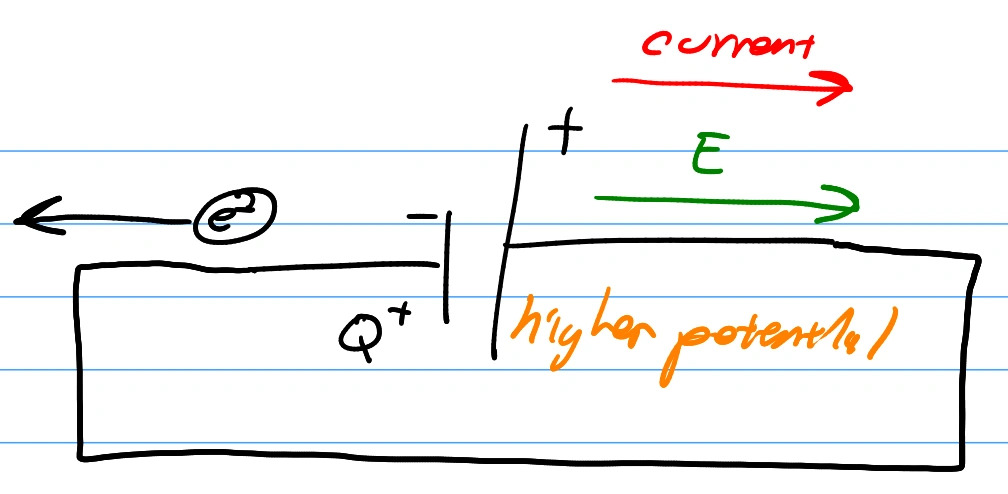
\includegraphics[width=8cm]{content/electromagnetism/battery-simple-circuit.jpg}

\subsection{Loop Law}

\begin{namedlaw}[Loop Law]
  In a circuit, the sum of the signed potential differences along the entire circuit is 0.

  \[
    \sum \Delta V = 0
  \]

  In a circuit with a battery, this means that the voltage (unsigned) of the battery is equal to the sum of the other potential differences along the circuit.
\end{namedlaw}

If a set of capacitors were replaced by a single capacitor without changing any of the observable properties of the circuit, then $C_\text{eq}$ (the \textbf{equivalent capacitance}) is equal to the capacitance of that single capcitor and $Q_\text{eq}$ (the \textbf{equivalent charge}) is equal to the capacitance of one plate of that single capacitor.

\begin{example}[Capacitors in parallel]
  \begin{align*}
    C_\text{eq} &= \sum C_i \\
    \mathcal{E} &= V_1 = \cdots = V_n \\
    Q_\text{eq} &= \sum Q_i
  \end{align*}
\end{example}

\begin{example}[Capacitors in series]
  \begin{align*}
    \frac{1}{C_\text{eq}} &= \sum \frac{1}{C_i} \\
    \mathcal{E} &= \sum V_i \\
    Q_\text{eq} &= Q_1 = \cdots = Q_n
  \end{align*}
\end{example}

\subsection{Current and resistance}

\begin{definition}[Current / amperage ($i$ or $I$)]
  The rate at which charges flow through a conductor.

  \[
    i = I = \frac{dq}{dt} \qquad \left(\Ampere = \frac{\Coulomb}{\second}\right)
  \]
\end{definition}

\begin{definition}[Junction]
  A place in a circuit at which the current can change.
\end{definition}

\begin{law}[Junction Rule]
  The sum of the current into a junction equals the sum of the current out of the junction.
  \[
    \sum I_\text{into} = \sum I_\text{out}
  \]
\end{law}

\begin{definition}[Current density]
  \[
    J = \frac{i}{A}
  \]
\end{definition}

\begin{definition}[Resistance ($R$)]
  \[
    R = \frac{V}{i} \qquad \left( \Ohm = \frac{\Volt}{\Ampere} \right)
  \]

  The resistance is a property of the conducting object.
\end{definition}

\begin{namedlaw}[Ohm's Law]
  \[
    V = iR
  \]
\end{namedlaw}

\begin{definition}[Resistivity]
  \[
    \rho = \frac{E}{J} \qquad
  \]

  The resistivity is a property of the conducting material.
\end{definition}

\begin{lemma}
  \[
    R = \frac{\rho \lambda}{A}
  \]
\end{lemma}

\begin{law}
  \[
    q = Ne
  \]
  where $N$ is the number of charge carriers.
\end{law}

\begin{definition}[Drift speed]
  \[
    v_\text{drift} = \frac{J}{ne}
  \]
  where $n = \frac{N}{\text{Volume}}$
\end{definition}

\begin{theorem}[Power consumed by a resistor]
  Most of this energy is converted to heat.
  \[
    P = IV = I^2 R = \frac{V^2}{R}
  \]
\end{theorem}

\begin{lemma}[Resistors in parallel]
  By the Loop Law,
  \[
    V_{eq} = V_1 = \cdots = V_n
  \]

  By the Junction Rule,
  \[
    \frac{\mathcal{E}}{R_{eq}} = i_{\text{total}} = \sum i_i
  \]

  Therefore by Ohm's Law,
  \[
    \frac{1}{R_{eq}} = \sum \frac{1}{R_i}
  \]
\end{lemma}

\begin{lemma}[Resistors in series]
  By the Loop Law,
  \[
    V_{eq} = \sum V_i
  \]

  Therefore by Ohm's Law,
  \[
    R_{eq} = \sum R_i
  \]
\end{lemma}

\subsection{RC circuits}

\begin{definition}[RC circuit]
  A circuit with a resistor and a capacitor.
\end{definition}

\begin{definition}[Time constant]
  For an RC circuit,
  \[
    \tau := R_{eq} C_{eq} \qquad (\second)
  \]
\end{definition}

\begin{law}[Charging a capacitor]
  A capacitor can be charged by applying an $\mathcal{EMF}$ such as a battery on both sides of the capacitor, possibly including a resistor or resistors with equivalent resistance $R$.

  Initial and final conditions:
  \begin{align*}
    t &= 0 & t &\to \infty \\
    q_0 &= 0 & q_{\text{max}} &= C\mathcal{E} \\
    i_0 &= \frac{\mathcal{E}}{R} & i_f &= 0 \\
  \end{align*}

  Applying the loop law:
  \[
    \mathcal{E} - R \frac{dq}{dt} - \frac{q}{c} = 0
  \]

  Solving the equation, we get:
  \begin{align*}
    q(t) &= q_{\text{max}} \left(1 - e^{- \frac{t}{\tau}}\right) \\
    i(t) &= i_0 e^{- \frac{t}{\tau}}
  \end{align*}
\end{law}

\begin{law}[Discharging a capacitor]
  A capacitor can be discharged by shorting both plates, possibly including a resistor or resistors with equivalent resistance $R$ in between.

  Initial and final conditions:
  \begin{align*}
    t &= 0 & t &\to \infty \\
    q_{\text{max}} &= C\mathcal{E} & q_f &= 0 \\
    i_0 &= -\frac{\mathcal{E}}{R} & i_f &= 0 \\
  \end{align*}

  Applying the loop law:
  \[
    - R \frac{dq}{dt} - \frac{q}{c} = 0
  \]

  Solving the equation, we get:
  \begin{align*}
    q(t) &= q_{\text{max}} e^{- \frac{t}{\tau}} \\
    i(t) &= i_0 e^{- \frac{t}{\tau}}
  \end{align*}

  (ensure $i_0 < 0$)
\end{law}

